\documentclass[11pt,a4paper]{article}
\usepackage[margin=1in]{geometry}
\usepackage{graphicx}
\usepackage{booktabs}
\usepackage{hyperref}
\usepackage{float}
\usepackage{caption}
\usepackage{subcaption}

\graphicspath{{reports/figures/}}

\title{Metal Peer-Group Risk Scoring\\Notebook Analysis Report}
\author{by Federico Lievano}
\date{\today}

\begin{document}
\maketitle

\begin{abstract}
This report summarizes the execution of four Jupyter notebooks and the shared
\texttt{notebook\_lib.py} module on a portfolio of 500 homeowners submissions from
\texttt{Results.csv}. The analysis covers data quality, peer-group percentile scoring,
synthetic submission simulation, and a supervised model benchmark (Ridge, ElasticNet,
Random Forest, KNN, Gradient Boosting, Logistic Regression). Figures are exported
automatically to \texttt{reports/figures/} when notebook cells run.
\end{abstract}

\section{Executive summary}

The portfolio is dominated by \textbf{Medium} risk band policies (87\%), with mean
peer-group score \textbf{38.9} on a 0--100 scale. Exposure (TIV) is the strongest
driver of portfolio-level score shifts; wildfire-only and roof-age stress tests move
the mean score only marginally on this book.

Supervised models approximate the holdout peer score with MAE around \textbf{7.6--8.0}
points. \textbf{Random Forest} achieves the lowest regression MAE; \textbf{Ridge} and
\textbf{ElasticNet} show the best alignment with lifetime claim counts (Spearman
$\approx 0.21$). None of the ML benchmarks replace the explainability of peer-group
percentiles for Metal submission triage.

\textbf{Recommendation:} use peer-group scoring as the primary triage layer; treat ML
models as offline benchmarks until underwriting and claim-outcome labels are available.

\section{Shared library: \texttt{notebook\_lib.py}}

\texttt{notebook\_lib.py} centralizes notebook logic:

\begin{itemize}
  \item \textbf{Data:} load \texttt{Results.csv} (with or without header row), deduplicate by \texttt{policy\_no} + \texttt{effective\_dt}, parse money and dates, build \texttt{clean\_*} numeric fields.
  \item \textbf{Peer groups:} keys from state, program type, product, and occupancy (e.g.\ \texttt{CA / Non-Admitted / HO / Primary}).
  \item \textbf{Scoring (3 layers):} absolute feature risk; global and peer-relative percentiles; similarity context via normalized features.
  \item \textbf{Explainability:} \texttt{build\_explanations()} returns per-variable percentiles and component contributions.
  \item \textbf{Simulation:} sample realistic synthetic rows from portfolio distributions, insert, and rescore.
  \item \textbf{ML benchmarks:} \texttt{run\_model\_comparison()} with 75/25 holdout; peer percentiles computed on train only.
  \item \textbf{Charts:} matplotlib helpers (\texttt{plot\_*}) save PNG to \texttt{reports/figures/} when cells execute.
\end{itemize}

\section{Notebook 01: Data understanding}

\subsection{Purpose}
Profile shape, nulls, deduplication, TIV and geographic mix.

\subsection{Results}
\begin{itemize}
  \item \textbf{500} rows, \textbf{111} columns; \textbf{0} duplicate policy+effective rows removed.
  \item \textbf{30} states; mean TIV \textbf{\$11.4M}, median \textbf{\$9.8M}.
\end{itemize}

\begin{figure}[H]
  \centering
  \begin{subfigure}{0.48\textwidth}
    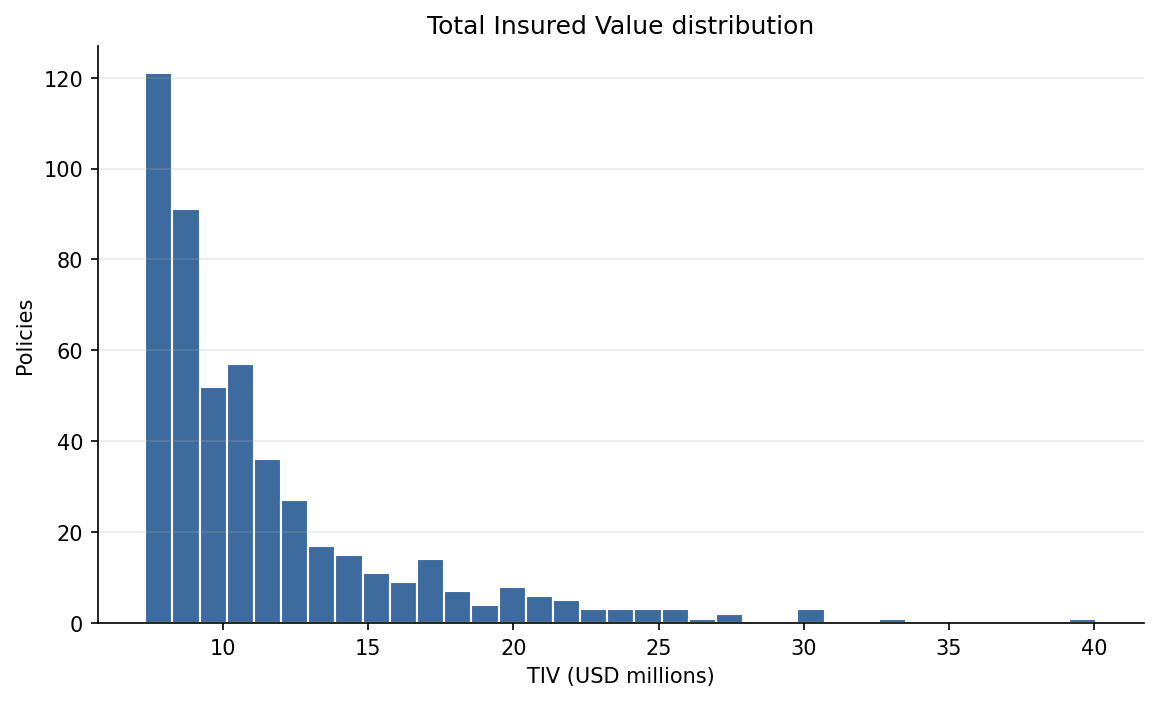
\includegraphics[width=\linewidth]{01_tiv_distribution.png}
    \caption{TIV distribution}
  \end{subfigure}\hfill
  \begin{subfigure}{0.48\textwidth}
    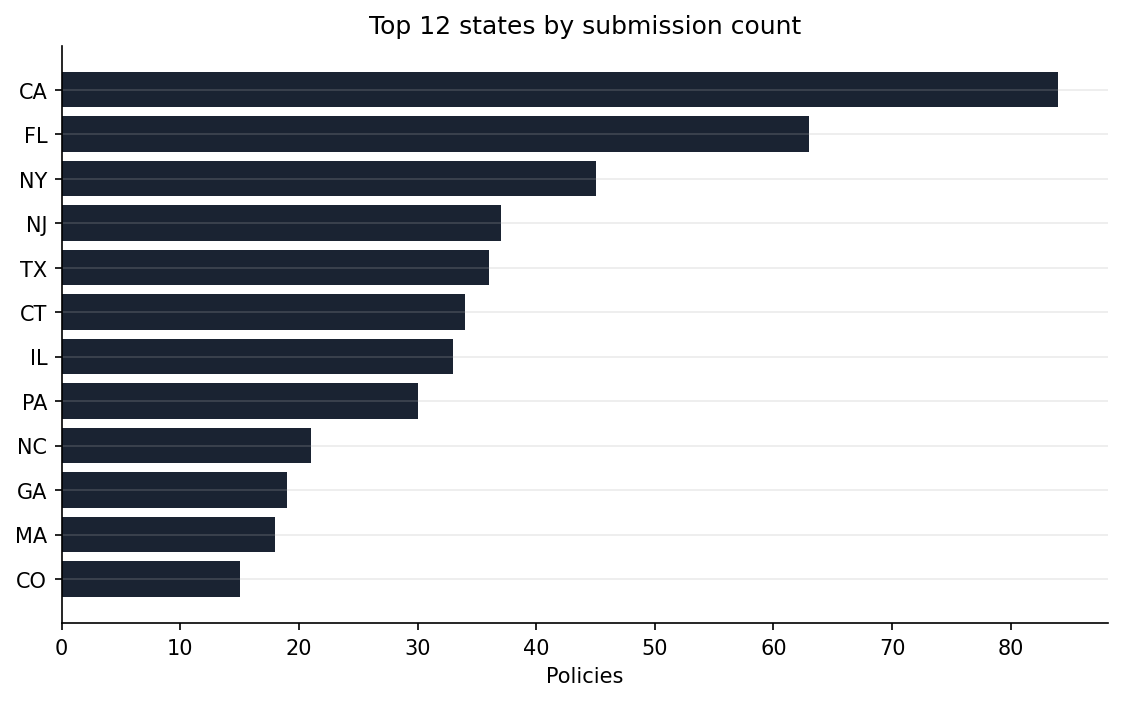
\includegraphics[width=\linewidth]{01_state_counts.png}
    \caption{Top states}
  \end{subfigure}
  \caption{Portfolio exposure and geography (Notebook 01).}
\end{figure}

The TIV distribution is right-skewed: a minority of very high TIV policies drives tail
risk. California, Florida, and New York dominate submission counts---consistent with
a non-admitted coastal and high-value book.

\section{Notebook 02: Peer-group scoring experiment}

\subsection{Purpose}
Score all submissions, inspect risk bands, and walk through low / medium / high examples.

\subsection{Results}
\begin{itemize}
  \item Mean score \textbf{38.9}; bands: Low \textbf{16}, Medium \textbf{436}, High \textbf{48}, Critical \textbf{0}.
  \item Lowest example: \texttt{HO200089145} (score \textbf{21.1}, MA / Admitted / HO / Primary).
  \item Highest example: \texttt{HO100022152-05} (score \textbf{66.9}, GA / Admitted / HO / Primary).
  \item Largest peer group: CA / Non-Admitted / HO / Primary (\textbf{77} policies).
\end{itemize}

\begin{figure}[H]
  \centering
  \begin{subfigure}{0.48\textwidth}
    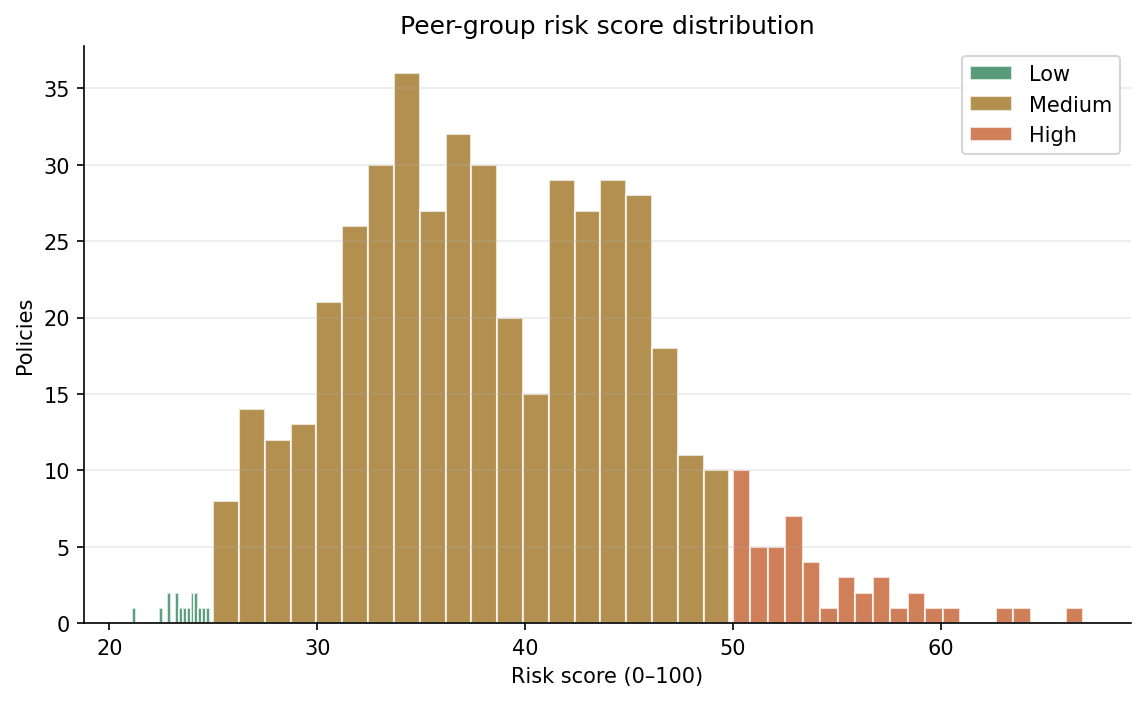
\includegraphics[width=\linewidth]{02_score_distribution.png}
    \caption{Score by band}
  \end{subfigure}\hfill
  \begin{subfigure}{0.48\textwidth}
    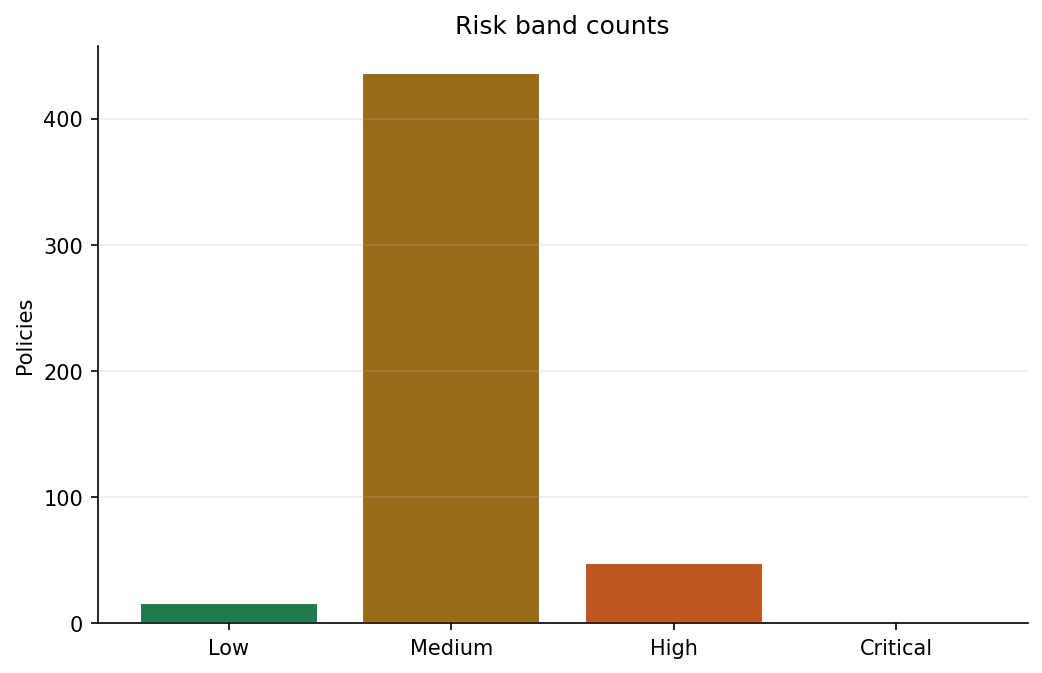
\includegraphics[width=\linewidth]{02_risk_bands.png}
    \caption{Band counts}
  \end{subfigure}
  \caption{Risk score distribution (Notebook 02).}
\end{figure}

\begin{figure}[H]
  \centering
  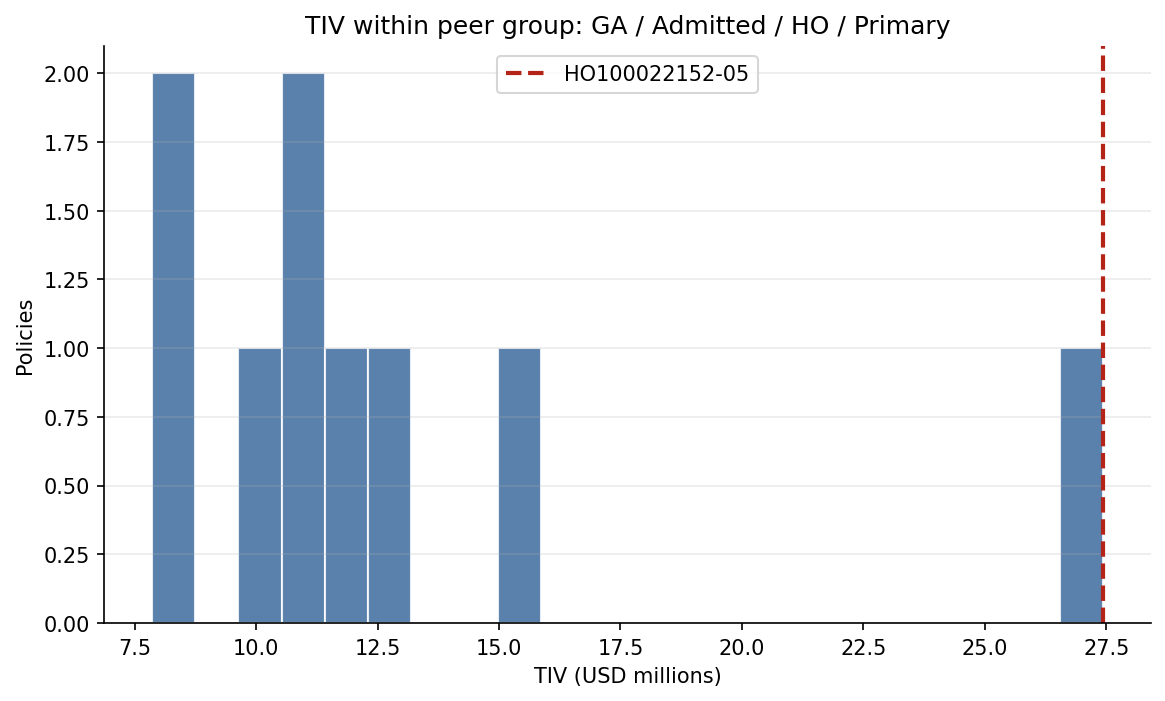
\includegraphics[width=0.85\textwidth]{02_peer_tiv_example.png}
  \caption{High-risk example: TIV vs peer group (GA / Admitted / HO / Primary). Selected policy sits in the upper tail of peer TIV.}
\end{figure}

The high example illustrates peer-relative logic: even within a single peer group, TIV
at the upper tail pushes exposure percentiles and the final score upward.

\section{Notebook 03: New submission simulation}

\subsection{Purpose}
Simulate a Metal-style upload: generate $\rightarrow$ insert $\rightarrow$ rescore $\rightarrow$ rank $\rightarrow$ nearest neighbors.

\subsection{Results (latest run)}
\begin{itemize}
  \item Simulated policy \texttt{SIM-3440F4D5}; score \textbf{49.7}; band \textbf{Medium}.
  \item Peer group: \texttt{PA / Non-Admitted / HO / Unknown}.
  \item Global rank \textbf{\#51} of \textbf{501} after insertion.
\end{itemize}

\begin{figure}[H]
  \centering
  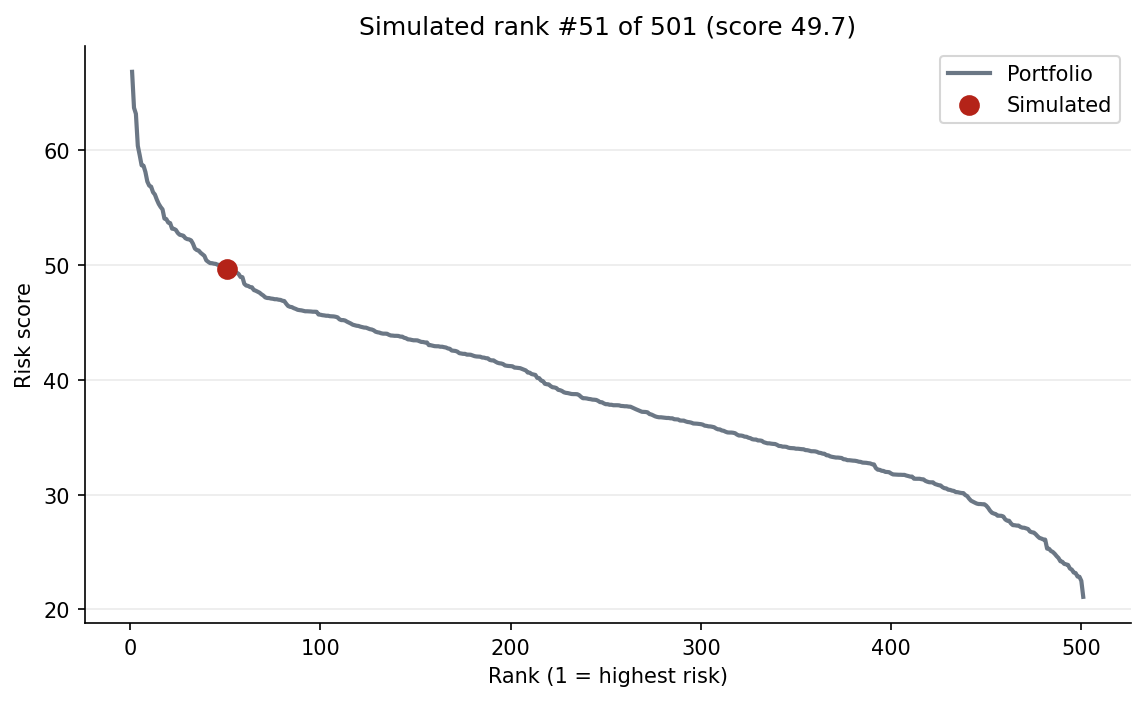
\includegraphics[width=0.85\textwidth]{03_simulation_rank.png}
  \caption{Simulated submission rank within the rescored portfolio (Notebook 03).}
\end{figure}

The simulated policy lands near the middle of the risk ranking---reasonable for a
random draw from portfolio marginals. In production, the same pipeline would run on
each new Metal submission before underwriting review.

\section{Notebook 04: Model validation and comparison}

\subsection{Purpose}
Sensitivity analysis and supervised benchmarks vs holdout peer-group score.

\subsection{Sensitivity}
\begin{table}[H]
  \centering
  \begin{tabular}{lc}
    \toprule
    Scenario & $\Delta$ mean score \\
    \midrule
    TIV +20\% & +0.568 \\
    Claims +20\% & +0.196 \\
    Wildfire score +20\% & +0.009 \\
    Roof age +5 years & +0.000 \\
    \bottomrule
  \end{tabular}
  \caption{Portfolio mean score shift under stress scenarios.}
\end{table}

\begin{figure}[H]
  \centering
  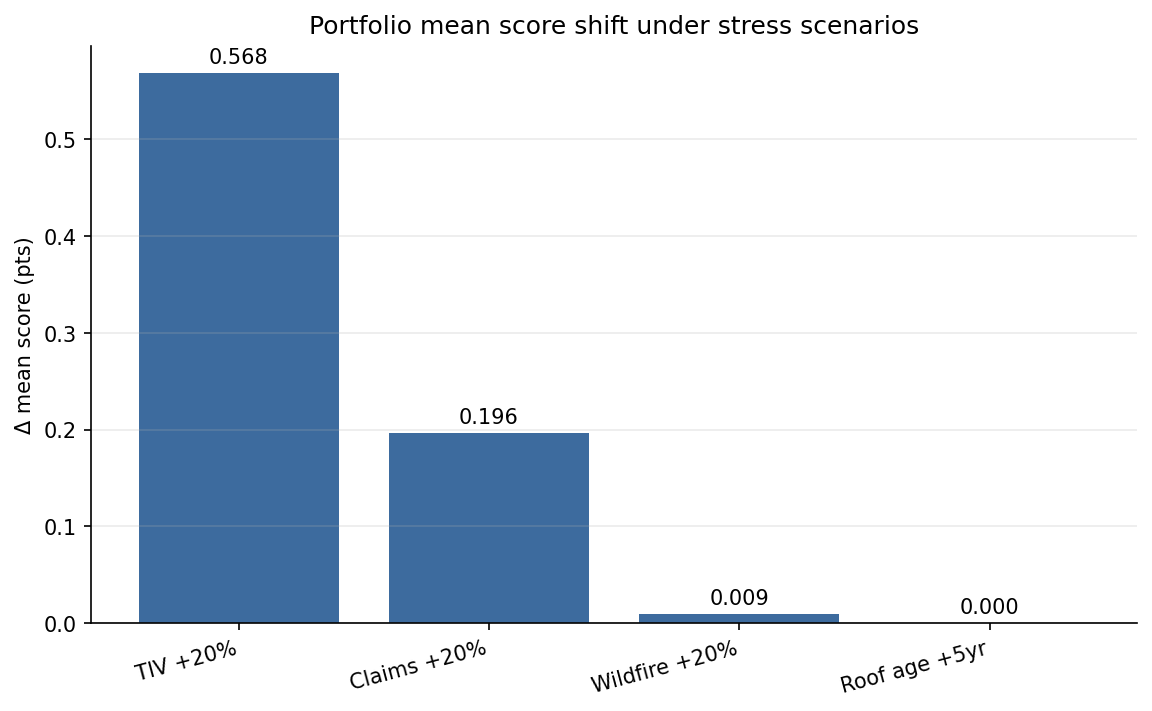
\includegraphics[width=0.75\textwidth]{04_sensitivity.png}
  \caption{Sensitivity chart (Notebook 04).}
\end{figure}

TIV dominates sensitivity on this dataset; wildfire and roof-age shocks are weak
because many policies lack populated wildfire scores or because roof age is already
encoded elsewhere.

\subsection{Regression benchmark (holdout $n=125$)}
\begin{table}[H]
  \centering
  \small
  \begin{tabular}{lcccc}
    \toprule
    Model & MAE & RMSE & $R^2$ & Spearman (claims) \\
    \midrule
    Peer-group (holdout) & 0.00 & 0.00 & 1.00 & 0.116 \\
    Random Forest & 7.65 & 9.23 & 0.086 & 0.068 \\
    Gradient Boosting & 7.90 & 9.71 & $-0.01$ & 0.024 \\
    ElasticNet & 7.95 & 9.86 & $-0.04$ & 0.210 \\
    KNN ($k{=}15$) & 7.98 & 9.56 & 0.019 & 0.021 \\
    Ridge & 7.98 & 9.94 & $-0.06$ & 0.212 \\
    \bottomrule
  \end{tabular}
  \caption{Regression vs holdout peer score (lower MAE is better).}
\end{table}

\begin{figure}[H]
  \centering
  \begin{subfigure}{0.48\textwidth}
    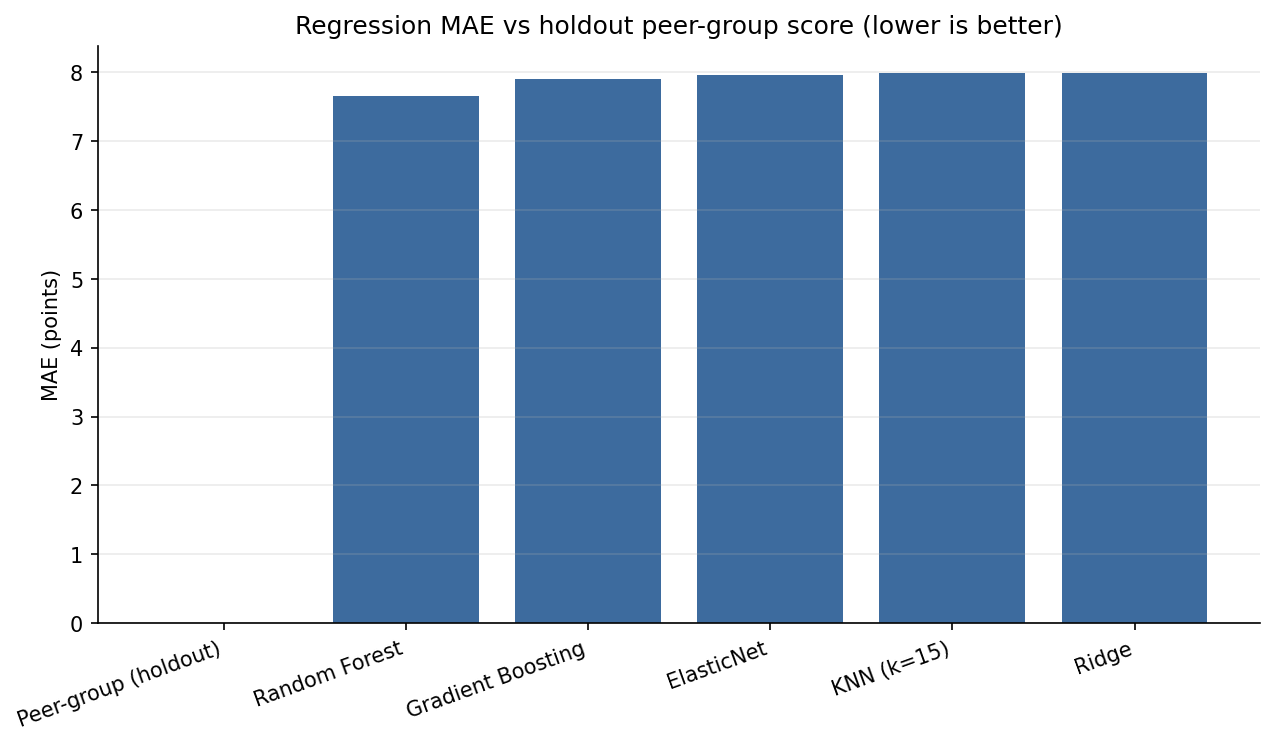
\includegraphics[width=\linewidth]{04_regression_mae.png}
    \caption{MAE by model}
  \end{subfigure}\hfill
  \begin{subfigure}{0.48\textwidth}
    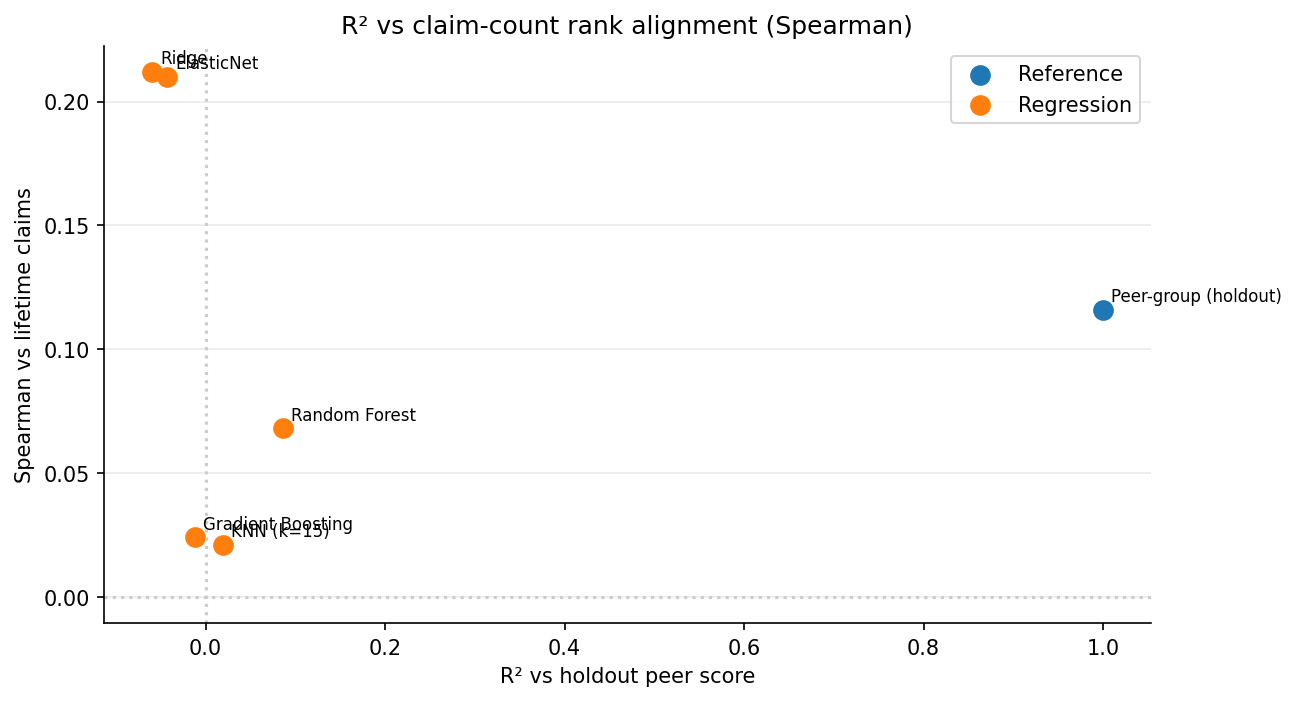
\includegraphics[width=\linewidth]{04_regression_scatter.png}
    \caption{$R^2$ vs claim alignment}
  \end{subfigure}
  \caption{Regression comparison (Notebook 04).}
\end{figure}

$R^2$ values are low because models predict a \emph{constructed} peer score, not claims.
Ridge/ElasticNet align better with claim-count ranks but do not beat peer scoring on MAE
by definition.

\subsection{Classification benchmark (high priority: score $\geq 50$)}
\begin{table}[H]
  \centering
  \small
  \begin{tabular}{lccc}
    \toprule
    Model & Accuracy & F1 & AUC \\
    \midrule
    Peer-group (holdout) & 1.000 & 1.000 & 1.000 \\
    Logistic Regression & 0.776 & 0.125 & 0.599 \\
    KNN ($k{=}15$) & 0.816 & 0.080 & 0.549 \\
    Random Forest & 0.816 & 0.000 & 0.488 \\
    \bottomrule
  \end{tabular}
  \caption{High-priority triage classification (higher AUC is better).}
\end{table}

\begin{figure}[H]
  \centering
  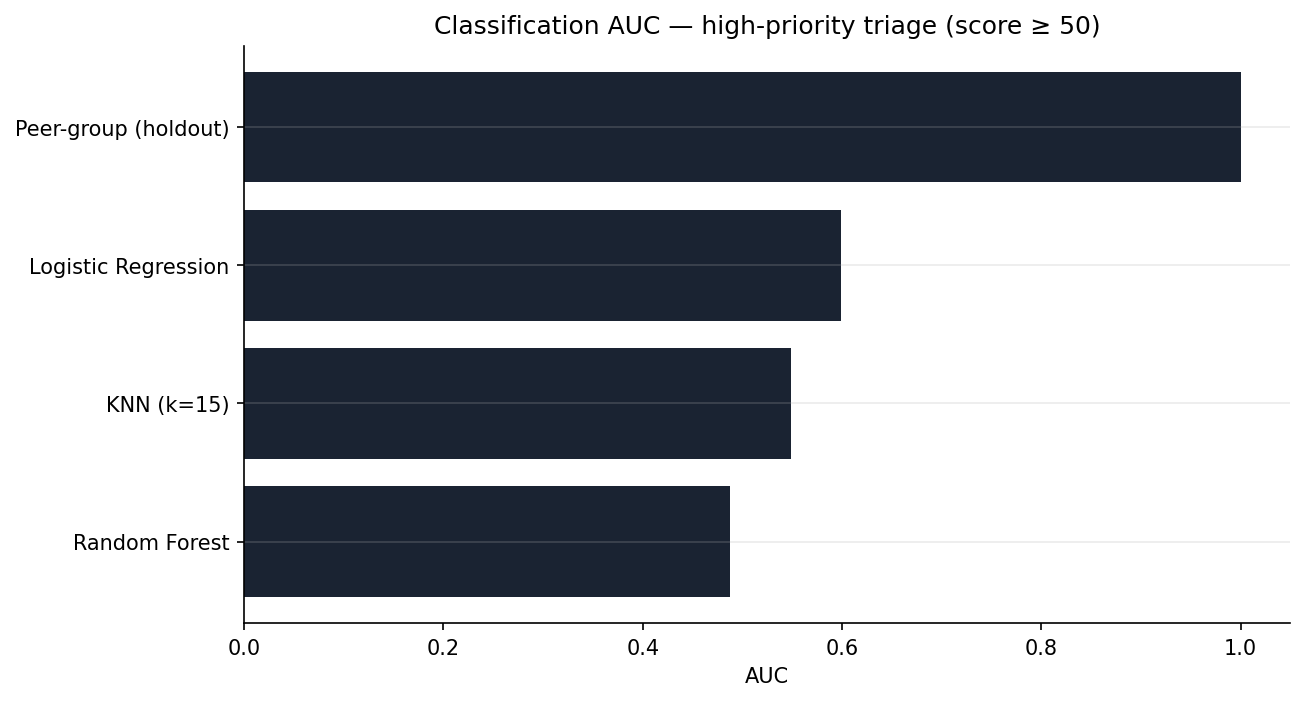
\includegraphics[width=0.75\textwidth]{04_classification_auc.png}
  \caption{Classification AUC (Notebook 04).}
\end{figure}

High accuracy with low F1 reflects class imbalance (few high-priority policies in the
test fold). Logistic Regression achieves the best ML AUC (\textbf{0.599}).

\subsection{Final comparison}
\begin{figure}[H]
  \centering
  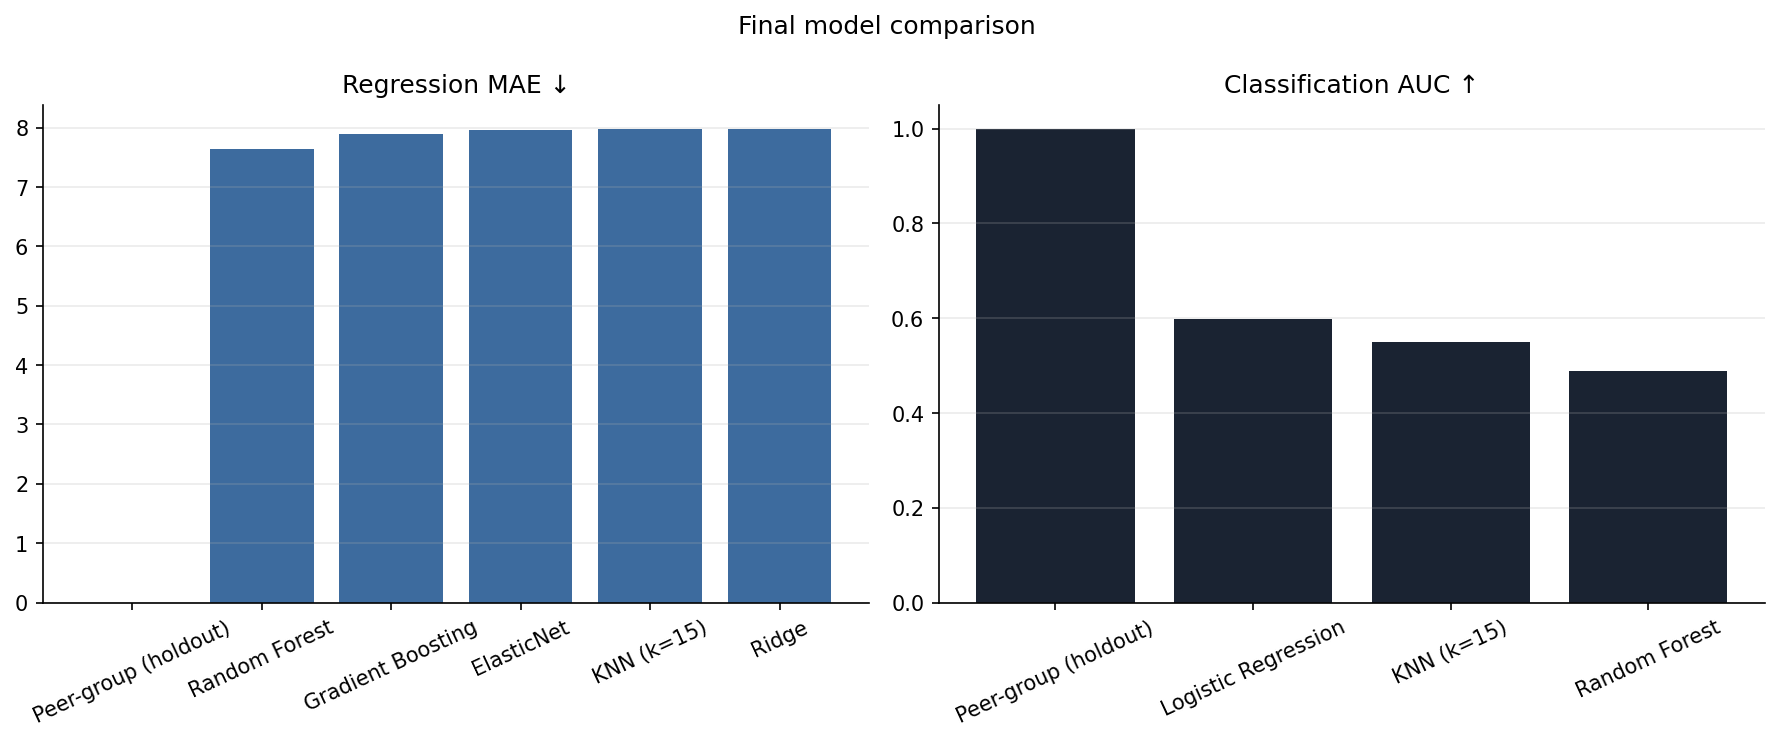
\includegraphics[width=0.95\textwidth]{04_final_comparison.png}
  \caption{Side-by-side MAE and AUC summary (Notebook 04).}
\end{figure}

\section{Conclusions}

\begin{enumerate}
  \item The book is \textbf{medium-risk on average} with a long right tail of high-TIV coastal and non-admitted business.
  \item \textbf{Peer-group scoring} is interpretable (state/program/product/occupancy percentiles) and stable for triage.
  \item \textbf{TIV and claims} are the main levers that move portfolio scores; CAT-only variables are secondary on this extract.
  \item \textbf{ML models} do not clearly outperform peer scoring on the holdout reference; linear models track claims slightly better but sacrifice peer-MAE fit.
  \item \textbf{Simulation} confirms the insert-and-rescore flow for future Metal integration.
\end{enumerate}

\section{Limitations and next steps}

\begin{itemize}
  \item No approve/decline or loss-ratio labels in \texttt{Results.csv}.
  \item Percentiles depend on reference population size and mix.
  \item Not a pricing or binding underwriting engine---risk prioritization only.
  \item \textbf{Next steps:} collect underwriting decisions and claims; calibrate weights with domain experts; expose scoring via API on Metal submission events.
\end{itemize}

\section{Overleaf usage}

Upload the \texttt{notebooks/} folder (or zip \texttt{notebooks.tex} + \texttt{reports/figures/*.png})
to Overleaf. Compile with pdfLaTeX. Figures are referenced as PNG only---no kaleido or PDF export required.

\end{document}
